\documentclass[conference]{IEEEtran}

\usepackage{cite}
\usepackage{amsmath,amssymb,amsfonts}
\usepackage{algorithmic}
\usepackage{graphicx}
\usepackage{textcomp}
\usepackage{xcolor}
\usepackage{hyperref}
\def\BibTeX{{\rm B\kern-.05em{\sc i\kern-.025em b}\kern-.08em
    T\kern-.1667em\lower.7ex\hbox{E}\kern-.125emX}}
\begin{document}

\title{Implementation of Sparse Graphical Memory for Robust Planning}

\author{\IEEEauthorblockN{Jie Wei Lek}
  \IEEEauthorblockA{\textit{CSD} \\
    \textit{SUTD}\\
    Singapore \\
    1005007}
}

\maketitle

\section{Introduction}
This document shall serve the purpose of detailing the author's simplified implementation of the Sparse Graphical Memory for Robust Planning in Robotics Operating System 2 (ROS2), and will be used for Singapore University of Technologty and Design (SUTD) Mobile Robotics Individual Project.

\section{Introduction to Sparse Graphical Memory (SGM)}

Currently there are two conventional approaches to reninforcement learning agents. (1) Deep Learning --- this method is good at learning from examples but does not scale with long-horizon tasks. (2) Classical Planning --- this method plans ahead in long-horizon tasks but fails to presume state space is generalised without raw sensory input.

This is where SGM would come in as an useful alternative. SGM is able to store observations as nodes and learaned distances as edges and feasible transitions in a sparse memory. This approach would aggregate states according to two-way consistency objective, whiles adapting classic state aggregation criteria to goal-conditioned objective.

\subsubsection{Two-Way Consistency --- Sparsity}
The formulas for two-way consistency can be denoted as:
\begin{equation}
  \max(w) \left| Q^{hl}(s_1, a=w | g) - Q^{hl}(s_2, a=wg) \right| \leq \tau_a
  \label{1}
\end{equation}
\begin{equation}
  \max(s_0) \left| Q^{hl}(s_0, a=w | g) - Q^{hl}(s_0, a=wg) \right| \leq \tau_a
  \label{2}
\end{equation}
This determines how nodes are merged together from a group of nodes to form these sparse nodes, which helps to minimise memory representation. They verify that both starting points and waypoints can be exchanged without altering the planner's behavior significantly, while making it more efficient.

\subsubsection{Cleanup}
Afterwards, lines between nodes that go through walls should be removed, since it is impossible for an entity to travel through the walls.

\subsubsection{Route Planning}
Finally, SGM would facilitate route planning by representing the environment as a sparse graph where nodes are represented by observations, and between them are edges that represent the feasible transitions between these states.


\section{Planned Proposal Summary}

In this report, the author shall implement features that SGM uses and simulate it using a custom robot and world in ROS2 and Gazebo.
The implementation shall be able to acheive the following.
\begin{enumerate}
  \item Create a custom robot and world in Gazebo.
  \item The world should also randomly create nodes and then perform sparsification and cleanup to find feasible edges
  \item The robot should then be able to navigate among different nodes and their edges using a navigation algorithm.
\end{enumerate}

\section{Implementation}
You may view the project's implementation source code \href{https://github.com/demeritbird/Sparse-Graphical-Memory-Robot-Planning}{here}. Detailed explanation on its installation and startup can also be found in there.

\subsection{Overall Project Architecture}
The project was created on ROS2 Humble on WSL2 Ubuntu 22.04.
The ROS2 workspace primary consists of 4 nodes:
\begin{enumerate}
  \item Robot description --- show robot's design
  \item Robot navigation --- contains core code for robot movement between ndoes
  \item Robot interfaces --- custom interface types to support robot movement
  \item Robot bringup --- launching robot in Gazebo world
\end{enumerate}

\subsection{Creating the Custom Robot}
The construction of the robot was mainly done using URDF and XACRO, which is shown in RViz (Fig. 1.). The robot was built with collision and inertia properties for the links and joints for testing purposes. For its movement I provided the robot's wheels with the \textit{diff\_drive\_controller} plugin. The robot was then launched in Gazebo aftewards, where a custom world was also created and launched (Fig. 2.).

I also created plugins for camera and laser scan.However, due to time constraints, they were not implemented further as additional features.

\begin{figure}[h]
  \centering
  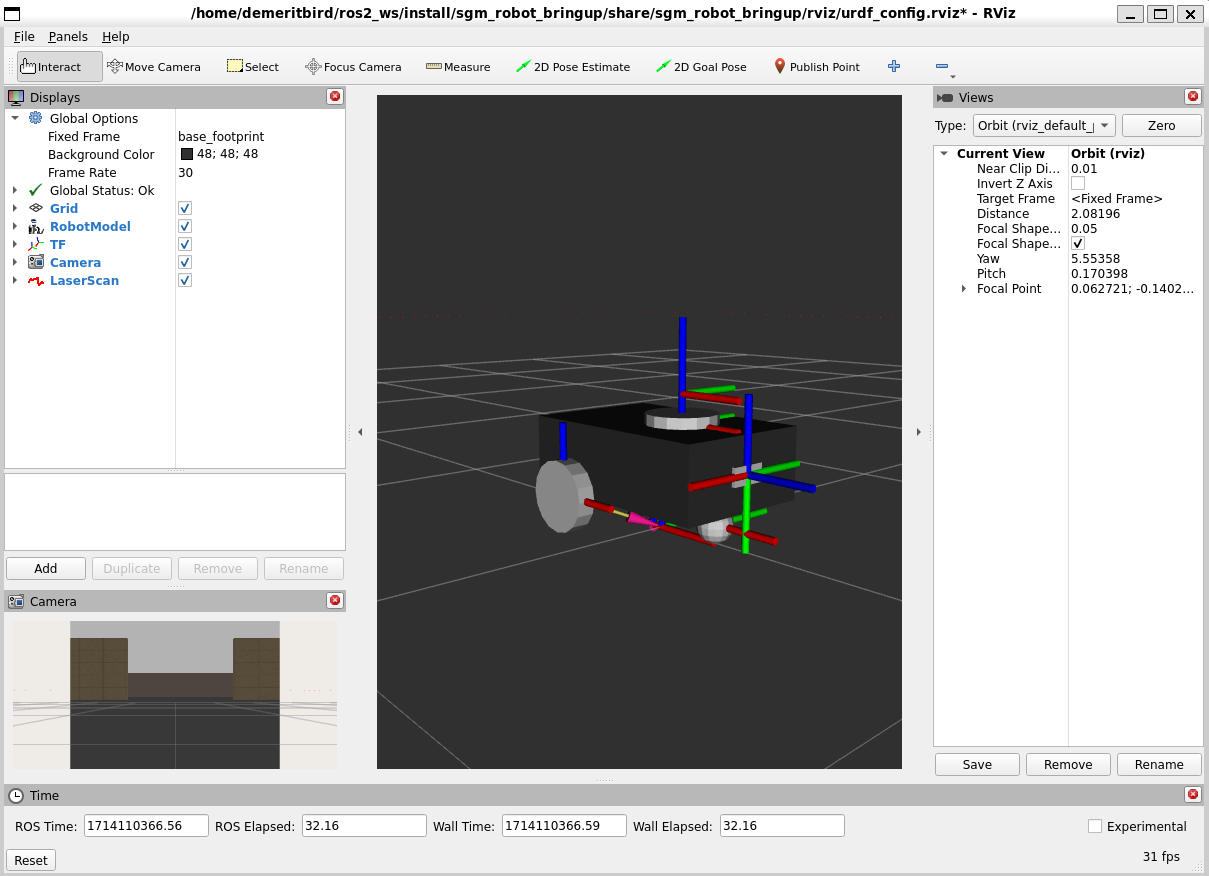
\includegraphics[width=0.5\textwidth]{../assets/robot_rviz.png}
  \caption{Custom robot as seen in RViz}
  \label{fig:example}
\end{figure}
\begin{figure}[h]
  \centering
  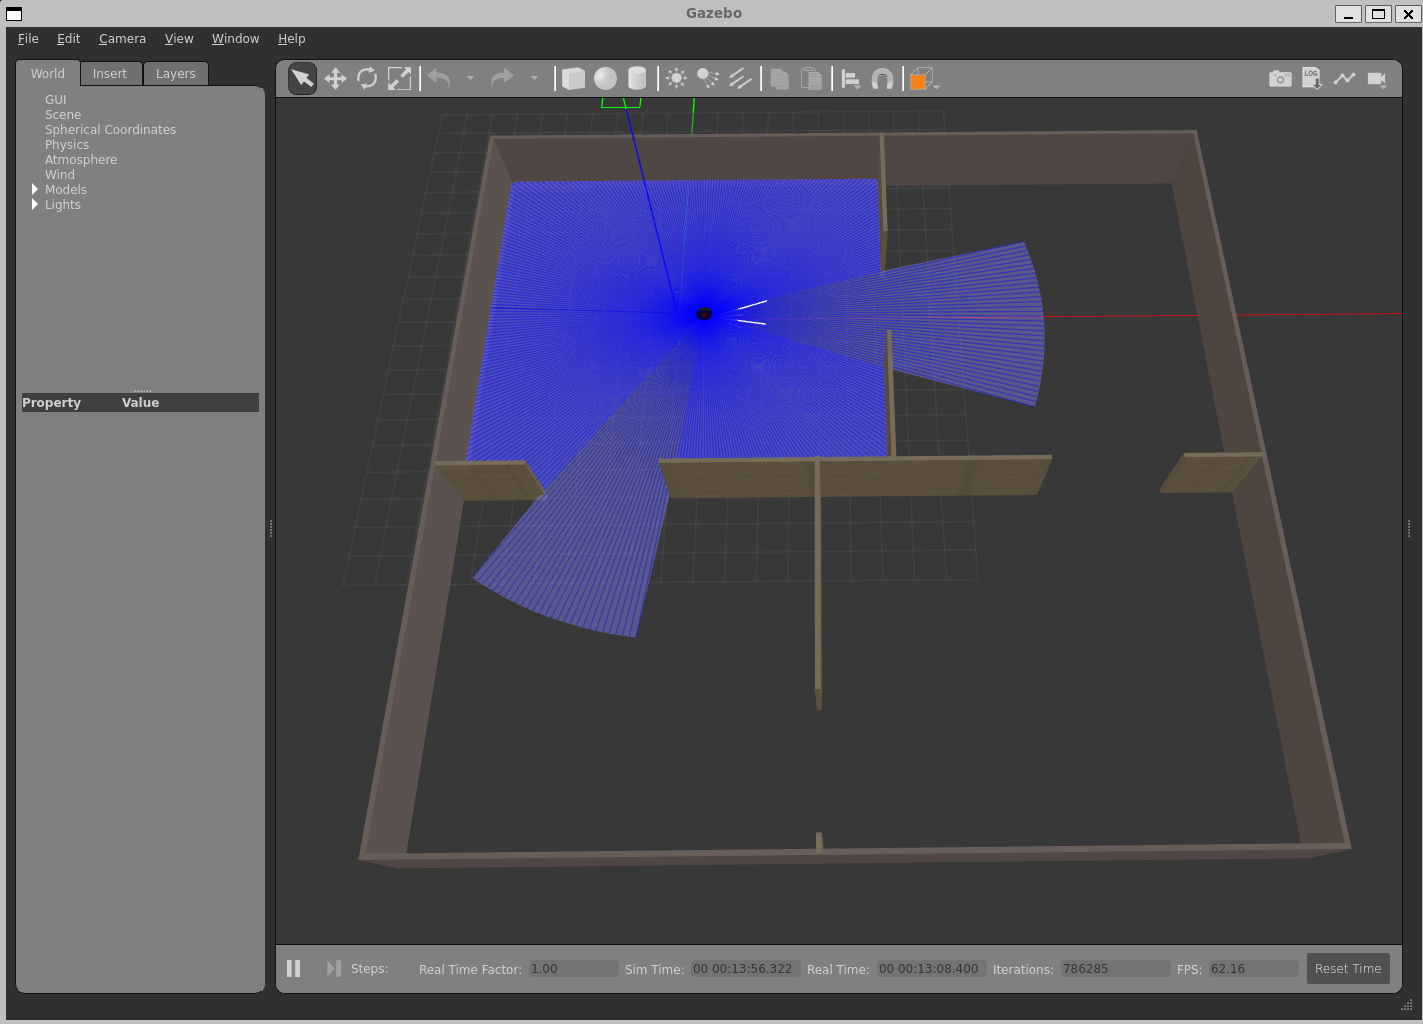
\includegraphics[width=0.5\textwidth]{../assets/robot_gazebo.png}
  \caption{Custom robot as seen in Gazebo}
  \label{fig:example}
\end{figure}

\subsection{Integrating Robot and Map}
With the robot and the map created, the robot needs to know where it is in our map. As such, I used SLAM toolkit and moved the robot around the map to allow the robot to understand the map information. In the map produced from SLAM toolkit, black pixels represent obstacles in the world (i.e. walls), and white spaces represent areas that robot can move around (Fig. 3.).
Due to time constraints, I decided to lean in on ROS' turtlebot's Navigation2 Stack instead of creating from scratch to assist in publishing our custom world's map information for the robot to consume later in the implementation. For the purposes of this project, I will only be using this navigation stack to get information about the map and not for its navigation features.

\begin{figure}[h]
  \centering
  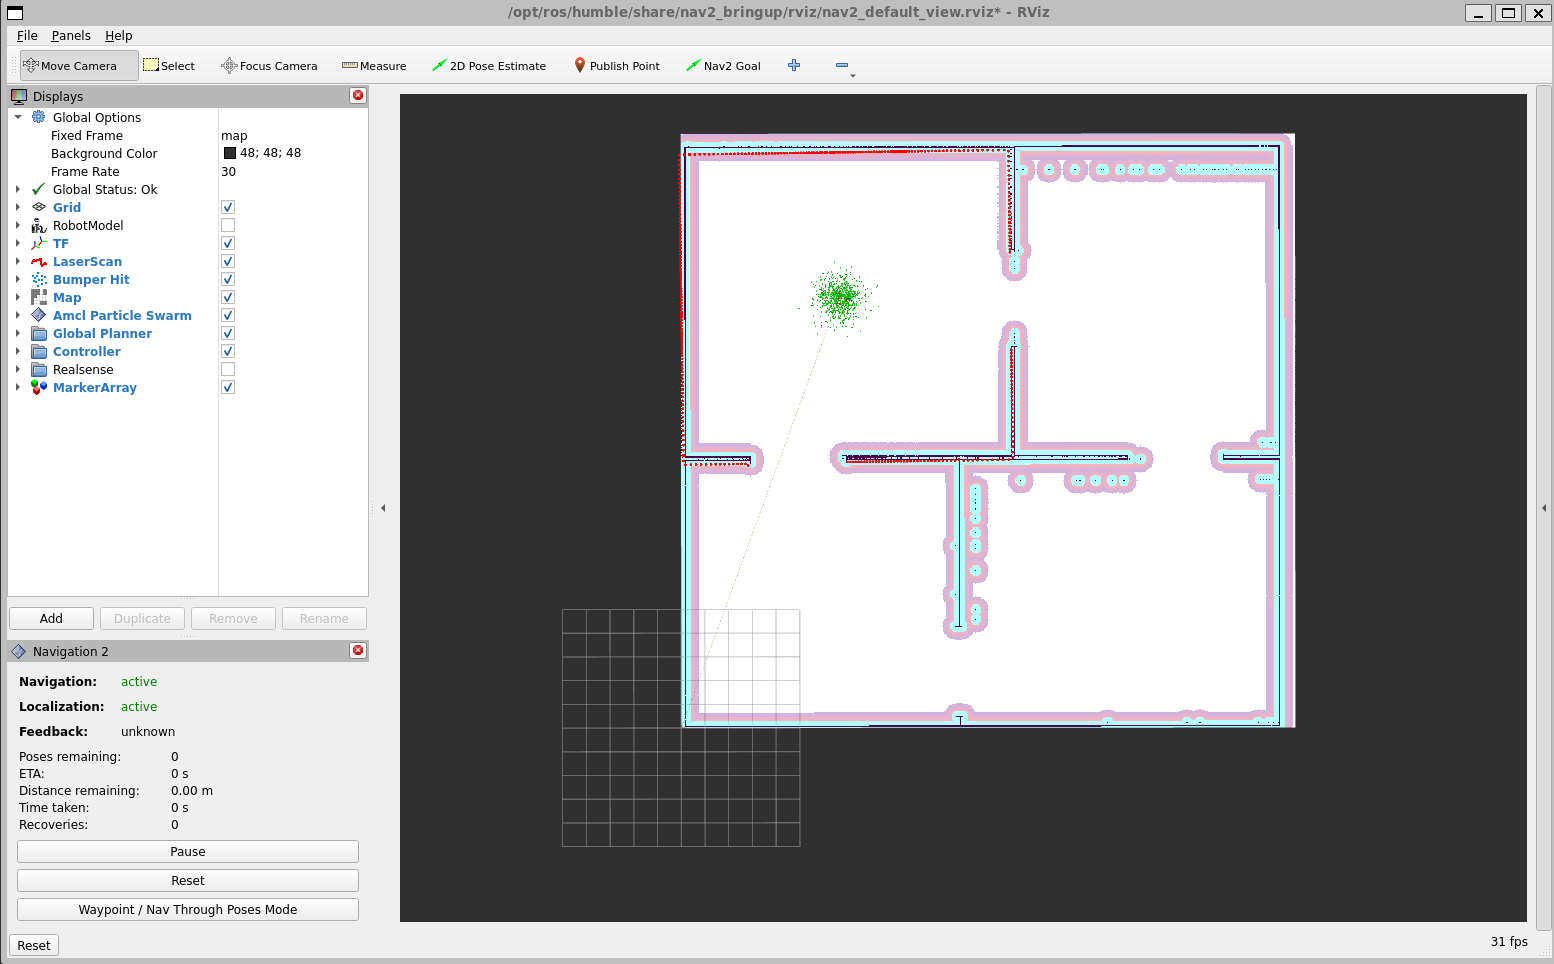
\includegraphics[width=0.5\textwidth]{../assets/map_nav_1.png}
  \caption{Robot as understood by the Navigation2 Stack. Robot locationa and orientation can be seen after initialisation.}
  \label{fig:example}
\end{figure}

\subsection{Generating and Plotting Points on World}
With the map information published, I am able to use it to generate random points on the map and merge them together using two-way consistency sparsification (Fig. 4.). From there, I can link nodes that are close to one another using threshold and detect feasible edges that do pass through walls which will consequentially be used during the final navigation process (Fig. 5.).

\begin{figure}[h]
  \centering
  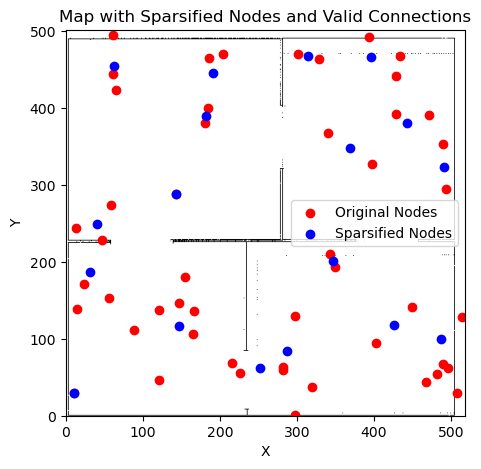
\includegraphics[width=0.5\textwidth]{../assets/map_nodes_1.png}
  \caption{Python simulation of how nodes would spawn on map (red), followed by sparsification of nodes (blue) using two-way consistency}
  \label{fig:example}
\end{figure}
\begin{figure}[h]
  \centering
  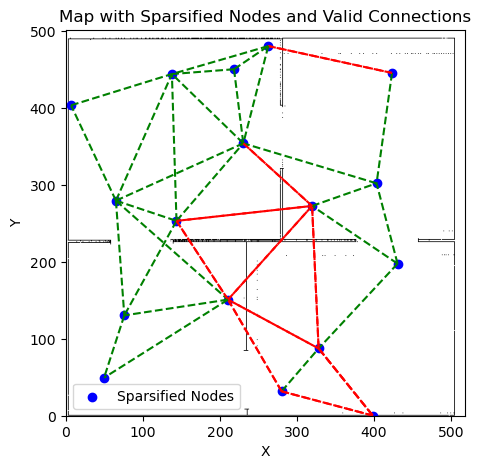
\includegraphics[width=0.5\textwidth]{../assets/map_nodes_2.png}
  \caption{Python simulation of another set of sparse nodes. Connected nodes via edges (green), edges that go through walls are non-feasible(red)}
  \label{fig:example}
\end{figure}

The visualisation of the nodes is then transferred over to RViz through publishing to the MarkerArray \textit{visualization\_marker\_array} topic (Fig. 6).
\begin{figure}[h]
  \centering
  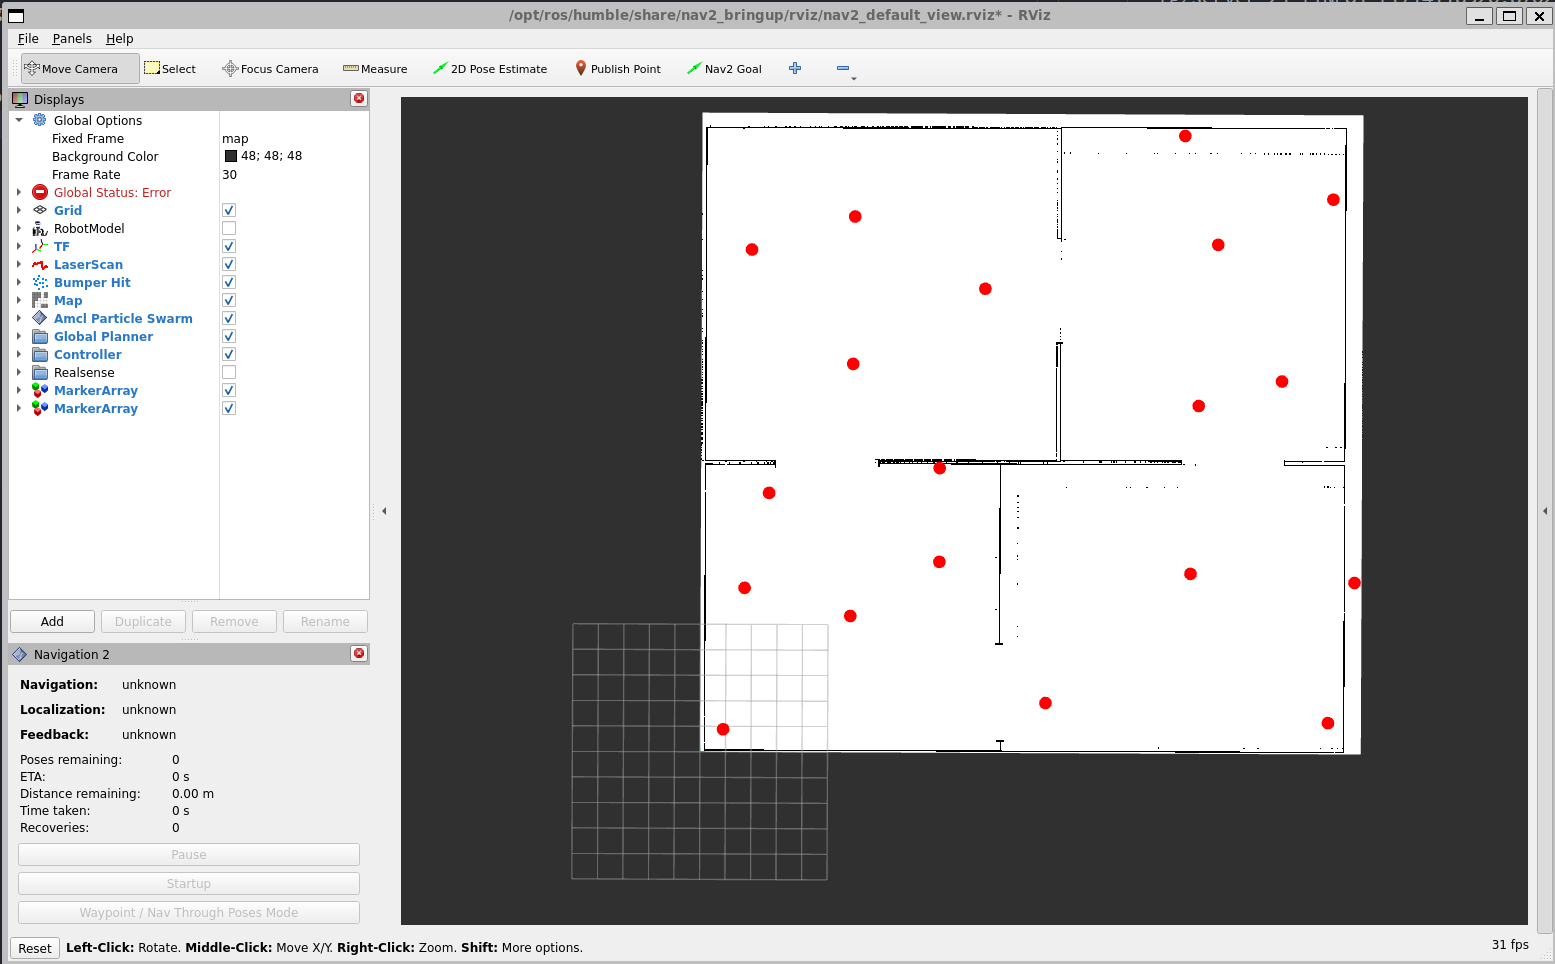
\includegraphics[width=0.5\textwidth]{../assets/map_nodes_3.png}
  \caption{Connected Nodes as seen in RViz.}
  \label{fig:example}
\end{figure}

\subsection{Robot Movement and Navigation}
In the implemented code, there are two major nodes for robot movement and navigation, \textit{marker\_points\_node} and \textit{robot\_controller\_server}.

\subsubsection{marker\_points\_node}
This ROS node subscribes and collects information about the map, processes the node mentioned earlier to get the sparse nodes and feasible edges, before publishes this new sparse node information to the RViz Visualisation as well as \textit{robot\_controller\_server}.

\subsubsection{robot\_controller\_server}
This ROS node is a multi-threaded ROS Action Server that first localises the robot in the map and moves it to the nearest available node for intialisation. It listens for future goals of new target sparse nodes to travel to, calculates the fastest way to get there through edges, and translates this information into commands for the robot to perform. These commands come in the form of the robot first rotating anti-clockwise to face its destination sparse node, then moving a linear distance, and stopping at its destination.

With these commands, the robot will then move from node to node to its destination node. In this implementation, since SGM is lenient on the navigation algorithm, I used the Breadth-First Search algorithm (BFS).

If the sparse node is unavailable to travel to (i.e. out-of-bounds), then the Server will reject this goal. The action server also comes with a feedback system to tell clients about which node location it will go to. The current goal policy for this server is to reject new goals if there is one in process, or if the robot is moving to its initial node location (Fig. 7).

\begin{figure}[h]
  \centering
  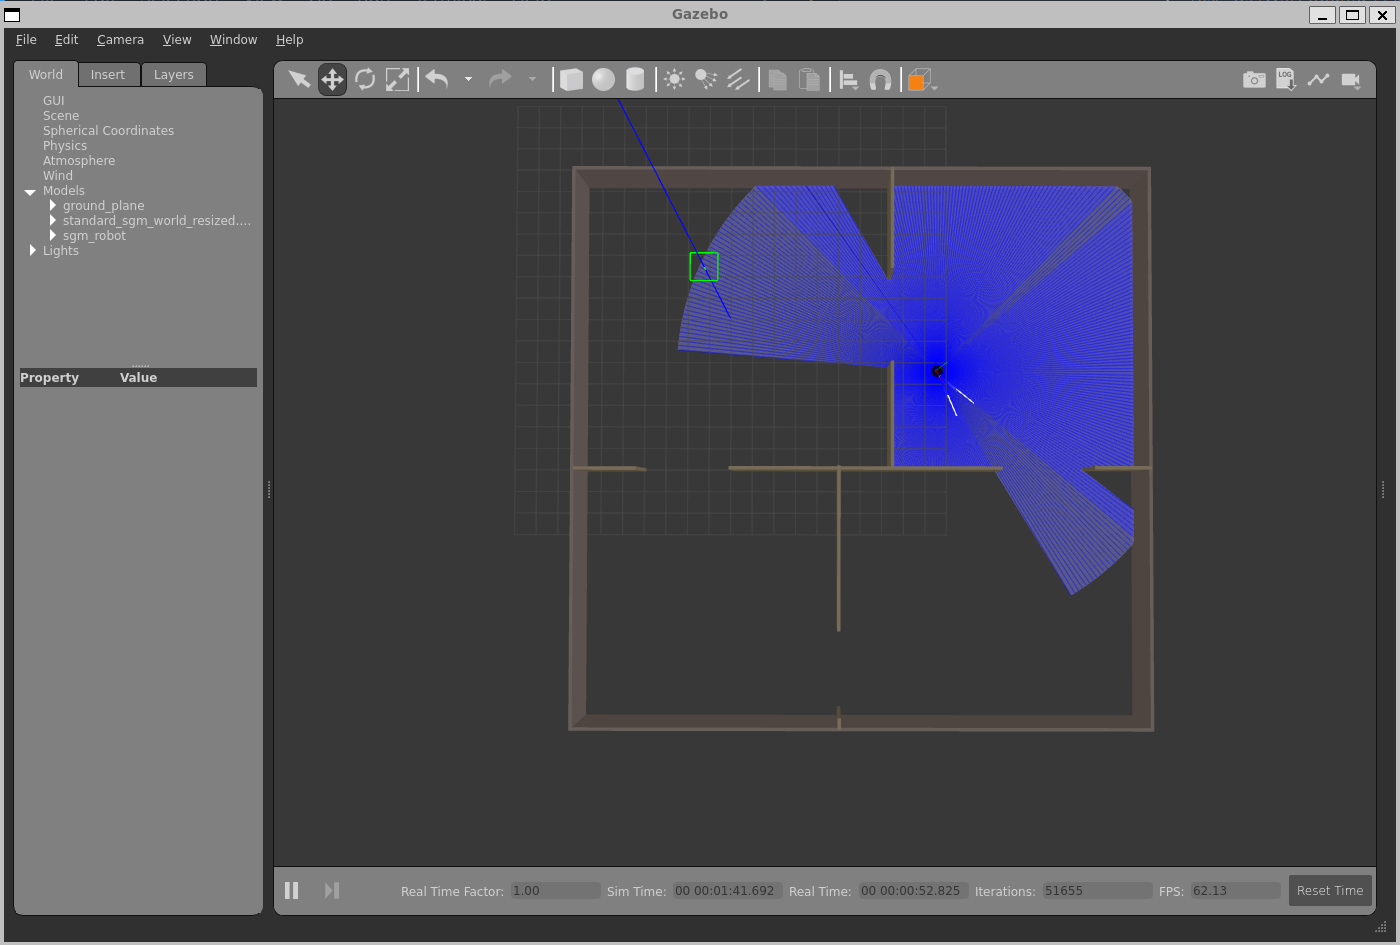
\includegraphics[width=0.5\textwidth]{../assets/map_nav_2.png}
  \caption{Robot moving in the custom world}
  \label{fig:example}
\end{figure}

\section{Evaluation and Limitations}
During the development process, the robot demonstrated the ability to correctly and autonomously navigate from one node to another using the fastest efficient route available. It is able to detect nodes reliably and plan efficiently. With its goal policy, it can also handle new target nodes dynamically as well.

However, given factors such as lags in computer processing and possibly vehicle friction, deviations occur in the rotation and advancement of the robot which compounded if the entire journey was long.

Additionally, while the navigation system effectively utilized the SGM representation for path planning, certain features and optimizations of SGM were not fully implemented, given time constraints. This includes improvements towards the memory construction of the robot between different state transitions dynamically to provide increased robustness of the robot, or unimplemented plugins that could error handle much effectively.

\begin{thebibliography}{00}
  \bibitem{b1} Emmons, Scott and Jain, Ajay and   Laskin, Michael and Kurutach, Thanard   and Abbeel, Pieter and Pathak, Deepak, Neural Information Processing Systems, Sparse Graphical Memory for Robust Planning. 2020.

\end{thebibliography}


\end{document}
